\documentclass[nooutcomes]{ximera}
\input{../preamble}


\author{Bobby Ramsey}
\license{Creative Commons Attribution 4.0 International License}
\acknowledgement{https://github.com/mooculus/calculusWithReview}

\title{Unit Circle}
% Learning Objectives for this section
%\begin{itemize}
%	\item Degrees and Radians
%	\item Reference Angles
%	\item The Definition of trigonometric functions in terms of the Unit Circle 
%	\item Evaluating trigonometric functions at standard angles
%\end{itemize}


\begin{document}

\begin{abstract}
	
\end{abstract}
\maketitle


%\typeout{************************************************}
%\typeout{Review Questions}
%\typeout{************************************************}

%\section{Review Materials}
%    \begin{itemize}[label=\textbullet]
%	\item \link[Combining Like Terms]{https://spot.pcc.edu/math/orcca/ed2/html/section-combining-like-terms.html}
%	\item \link[Algebraic Properties and Simplifying Expressions]{https://spot.pcc.edu/math/orcca/ed2/html/section-algebraic-properties-and-simplifying-expressions.html}
%   \end{itemize}
\begin{motivatingQuestions}\begin{itemize}
	%Often start a section. 
	\item How can we define trigonometric functions for angles that do not come from triangles?
\end{itemize}\end{motivatingQuestions}

\section{Introduction}

In the previous sections, you were introduced to the basic trigonometric functions sine and cosine, and saw how they relate measures of angles to
measurements of triangles. Given a right triangle
\begin{image}[2in]
  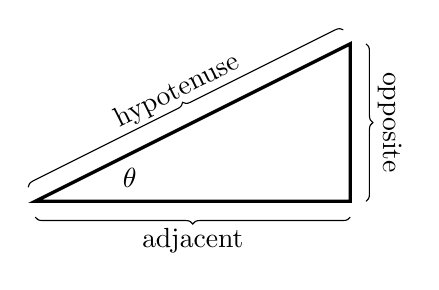
\begin{tikzpicture}
    \coordinate (C) at (0,2);
    \coordinate (D) at (4,2);
    \coordinate (E) at (4,4);
   % \tkzMarkRightAngle(C,D,E)
   % \tkzMarkAngle(D,C,E)
    \draw[decoration={brace,mirror,raise=.2cm},decorate,thin] (0,2)--(4,2);
    \draw[decoration={brace,mirror,raise=.2cm},decorate,thin] (4,2)--(4,4);
    \draw[decoration={brace,raise=.2cm},decorate,thin] (0,2)--(4,4);
    \draw[very thick] (D)--(E)--(C)--cycle;
    \node at (2,2-.5) {adjacent};
    \node[rotate=-90] at (4+.5,3) {opposite};
    \node[rotate=26.5] at (2-.2,3+.4) {hypotenuse};
    \node at (1.2,2.3) {$\theta$};
  \end{tikzpicture}
\end{image}
we define
\[
\cos(\theta) =
\frac{\text{adjacent}}{\text{hypotenuse}}\qquad\text{and}\qquad\sin(\theta)
= \frac{\text{opposite}}{\text{hypotenuse}}.
\]

There is a limitation in this, which you may have noticed. We can only build a triangle with a base angle $\theta$ if $\theta$ is between $0^\circ$ and $90^\circ$. We work now to rectify this deficiency.

\section{The Unit Circle}
		

First, note that the values of sine and cosine do not depend on the scale of the
triangle. Being very explicit, if we take our triangle and scale it up by a factor of $k$ (multiplying each side length by $k$) we obtain

\begin{image}[2in]
      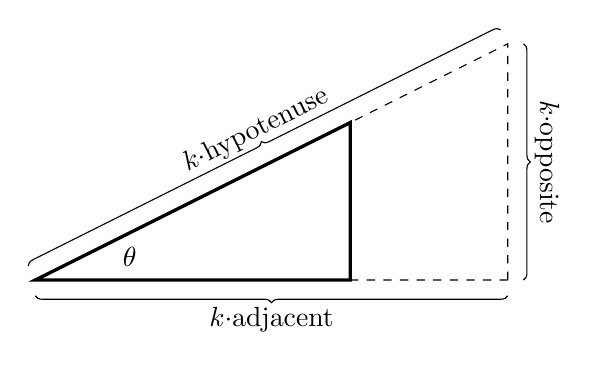
\begin{tikzpicture}
      \coordinate (A) at (6,2);
      \coordinate (B) at (6,5);
      \coordinate (C) at (0,2);
      \coordinate (D) at (4,2);
      \coordinate (E) at (4,4);
      %\tkzMarkRightAngle(C,A,B)
      %\tkzMarkRightAngle(C,D,E)
      %\tkzMarkAngle(D,C,E)
      
      
      \draw[decoration={brace,mirror,raise=.2cm},decorate,thin] (0,2)--(6,2);
      \draw[decoration={brace,mirror,raise=.2cm},decorate,thin] (6,2)--(6,5);
      \draw[decoration={brace,raise=.2cm},decorate,thin] (0,2)--(6,5);
      \draw[dashed] (A)--(B)--(C)--cycle;
      \draw[very thick] (D)--(E)--(C)--cycle;
      \node at (3,2-.5) {\text{$k\cdot$adjacent}};
      \node[rotate=-90] at (6+.5,3.5) {$k\cdot$opposite};
      \node[rotate=26.5] at (3-.2,3.5+.4) {$k\cdot$hypotenuse};
      \node at (1.2,2.3) {$\theta$};
      \end{tikzpicture}
\end{image}
\[
\cos(\theta) = \frac{k\cdot\text{adjacent}}{k\cdot\text{hypotenuse}} =\frac{\text{adjacent}}{\text{hypotenuse}}
\]
and
\[
\sin(\theta) = \frac{k\cdot\text{opposite}}{k\cdot\text{hypotenuse}} = \frac{\text{opposite}}{\text{hypotenuse}}.
\]
Notice that the \emph{ratios} of the corresponding side lengths are not changed. The individual side lengths are changed, but the ratios are preserved.


Because of this we could simply assume that whenever we draw a triangle
for computing sine and cosine, that the hypotenuse will have length $1$ (by dividing each side by the length of the hypotenuse). 
We can do this because we are simply scaling the triangle, and as we see
above, this makes absolutely no difference when computing sine and
cosine. When the hypotenuse is $1$, we find that a convenient
way to think about sine and cosine is via a circle.
\begin{image}
\begin{tikzpicture}
	\begin{axis}[
            xmin=-1.1,xmax=1.1,ymin=-1.1,ymax=1.1,
            axis lines=center,
            width=4in,
            xtick={-1,1},
            ytick={-1,1},
            clip=false,
            unit vector ratio*=1 1 1,
            xlabel=$x$, ylabel=$y$,
            every axis y label/.style={at=(current axis.above origin),anchor=south},
            every axis x label/.style={at=(current axis.right of origin),anchor=west},
          ]        
          \addplot [dashed, smooth, domain=(0:360)] ({cos(x)},{sin(x)}); %% unit circle

        \end{axis}
\end{tikzpicture}
\end{image}
We call this the \emph{unit circle}. 
\begin{definition}
	The \dfn{Unit Circle} is the circle of radius $1$, with center at the origin. It is the graph of the equation $x^2 + y^2 = 1$.
\end{definition}

An angle $\theta$ is in \emph{standard position} if the vertex of the angle is at the origin and one side oriented along the positive $x$-axis. The ray along the positive $x$-axis is called the \emph{initial side} of the angle, and the
other ray is called the \emph{terminal side} of the angle. The angle can be thought of as the counter-clockwise rotation necessary to spin the initial side to the terminal side. 


%\begin{minipage}{.5\textwidth}
	\begin{image}
	\begin{tikzpicture}
		\begin{axis}[
	            xmin=-1.1,xmax=1.1,ymin=-1.1,ymax=1.1,
	            axis lines=center,
	            width=4in,
	            xtick={-1,1},
	            ytick={-1,1},
	            clip=false,
	            unit vector ratio*=1 1 1,
	            xlabel=$x$, ylabel=$y$,
	            every axis y label/.style={at=(current axis.above origin),anchor=south},
	            every axis x label/.style={at=(current axis.right of origin),anchor=west},
	          ]        
	          \addplot [dashed, smooth, domain=(0:360)] ({cos(x)},{sin(x)}); %% unit circle
	
	          \addplot+[penColor2,->] plot coordinates {(0,0) (.766,.643)}; %% 40 degrees
	
	%          \addplot [ultra thick,penColor] plot coordinates {(.766,0) (.766,.643)}; %% 40 degrees
	          \addplot+ [ultra thick,penColor, ->] plot coordinates {(0,0) (1,0)}; %% 40 degrees
	          
	          \addplot [textColor,smooth, domain=(0:40)] ({.15*cos(x)},{.15*sin(x)});
	          \node at (axis cs:.15,.07) [anchor=west] {$\theta$};
	%          \node[penColor, rotate=-90] at (axis cs:.84,.322) {$\sin(\theta)$};
	          \node[penColor] at (axis cs:.5,0) [anchor=north] {Initial Side};
	          \node[penColor2, rotate=40] at (axis cs:0.383,0.5) [anchor=north] {Terminal Side};
	         \end{axis}
	\end{tikzpicture}
	\end{image}
%\end{minipage}% This must go next to `\end{minipage}`
%\begin{minipage}{.5\textwidth}
	\begin{image}
	\begin{tikzpicture}
		\begin{axis}[
	            xmin=-1.1,xmax=1.1,ymin=-1.1,ymax=1.1,
	            axis lines=center,
	            width=4in,
	            xtick={-1,1},
	            ytick={-1,1},
	            clip=false,
	            unit vector ratio*=1 1 1,
	            xlabel=$x$, ylabel=$y$,
	            every axis y label/.style={at=(current axis.above origin),anchor=south},
	            every axis x label/.style={at=(current axis.right of origin),anchor=west},
	          ]        
	          \addplot [dashed, smooth, domain=(0:360)] ({cos(x)},{sin(x)}); %% unit circle
	
	          \addplot+[penColor2,->] plot coordinates {(0,0) (.766,.643)}; %% 40 degrees
	
	         \addplot+ [ultra thick,penColor, ->] plot coordinates {(0,0) (1,0)}; %% 40 degrees
	          
	          \addplot [textColor,smooth, domain=(0:400)] ({(.15*(1+x/400))*cos(x)},{(.15*(1+x/400))*sin(x)});
	          
	          \node at (axis cs:.15,.07) [anchor=west] {$\phi$};
	         \end{axis}
	\end{tikzpicture}
	\end{image}
%\end{minipage}

Notice that the angles $\theta$ and $\phi$ from the two images above both rotate the initial side of the angle to the same terminal side, but the angle $\phi$ wraps around the origin first. Two angles are \emph{coterminal} if they have the same terminal side.
The angles $\theta$ and $\phi$ are coterminal. 

You can also think about an angle wrapping two, three, or four times before 
getting to the terminal side. You can also think about rotating clockwise instead of counter-clockwise. We consider counter-clockwise the positive direction, and clockwise the negative direction for angles. 

\begin{example}
	Find two angles that are coterminal with $30^\circ$, one positive and one negative.

	\begin{explanation}

		If we start with $30^\circ$, and then take another complete counter-clockwise rotation ($360^\circ$), we end up at $390^\circ$. That means $390^\circ$ is coterminal with $30^\circ$.

		If we start with $30^\circ$, and then take another complete clockwise rotation ($-360^\circ$), we end up at $30^\circ-360^\circ = -330^\circ$. That means $-330^\circ$ is coterminal with $30^\circ$.
	\end{explanation}
\end{example}



\section{Radians}

In everyday life, we typically measure angles in degrees. You will see in Calculus that using degrees can lead to a lot of complications. There is a better choice, more closely related to the geometry of the circle.
Notice that an angle identifies an arc along the circumerence of the unit circle? We'll call the arc constructed this way the \emph{subtended arc}.


\begin{image}
\begin{tikzpicture}
	\begin{axis}[
            xmin=-1.1,xmax=1.1,ymin=-1.1,ymax=1.1,
            axis lines=center,
            width=4in,
            xtick={-1,1},
            ytick={-1,1},
            clip=false,
            unit vector ratio*=1 1 1,
            xlabel=$x$, ylabel=$y$,
            every axis y label/.style={at=(current axis.above origin),anchor=south},
            every axis x label/.style={at=(current axis.right of origin),anchor=west},
          ]        
          \addplot [dashed, smooth, domain=(0:360)] ({cos(x)},{sin(x)}); %% unit circle

          \addplot+[penColor2,->] plot coordinates {(0,0) (.766,.643)}; %% 40 degrees

          \addplot+ [ultra thick,penColor, ->] plot coordinates {(0,0) (1,0)}; %% 40 degrees
          
          \addplot [textColor,smooth, domain=(0:40)] ({.15*cos(x)},{.15*sin(x)});
          \node at (axis cs:.15,.07) [anchor=west] {$\theta$};
          \addplot [penColor3,smooth, ultra thick, domain=(0:40)] ({cos(x)},{sin(x)});
          \addplot[penColor3, soliddot] coordinates { (.766,.643)}; %% 40 degrees
          \addplot[penColor3, soliddot] coordinates {(1,0)}; %% 40 degrees                    
          \node at (axis cs:.95,.37) [penColor3, right] {$S$};
         \end{axis}
\end{tikzpicture}
\end{image}

Notice that as $\theta$ grows (counter-clockwise) from $0^\circ$ the length of this arc, called $S$, also grows. 

\begin{example}
	If $\theta$ is a right angle, calculate the length $S$.
	
	\begin{explanation}

		If $\theta = 90^\circ$, the arc is a quarter of the circle. The circumference of the circle is $C = 2\pi r = 2\pi (1) = 2\pi$. Since $S$ will be a quarter of that,	$S = \frac{1}{4}(2\pi) = \frac{\pi}{2}$.
	\end{explanation}
\end{example}

The units we will be measuring angles, \emph{radians}, is actually based on arc lengths like this.
\begin{definition}
	One \dfn{radian} is the angle which, in standard position, subtends an arc of length $1$.
\end{definition}

That is, an angle measuring $1$ radian has $S = 1$. Let us suppose that the radius of the circle, and therefore the length of the subtended arc, has units.
This means that an angle $\theta$ of $1$ radian, in a circle of radius $1$ unit, subtends an arclength of $S = 1$ unit. We know that the formula for 
arclength is given by $S = R \theta$, so that $\theta = \dfrac{S}{R}$. That means $1$ radian is equal to $\dfrac{1 \textrm{unit}}{1 \textrm{unit}}$. 
Notice that the ``units'' cancel out? That means \textbf{radians are a unitless unit}. When our angle is measured in radians, that angle is really just
a number.


In one complete revolution ($360^\circ$) we have subtended the entire circle so $S = 2\pi$. 
Based on this and the definition of the radian above, 
one complete revolution measures $2\pi$ radians. That is an angle measuring $360^\circ$ measures $2\pi$ radians. This gives us a way to convert between degrees and radians! Note that $\frac{360}{2\pi}$ can be reduced to $\frac{180}{\pi}$.
\begin{callout}
	\begin{itemize}
		\item To convert from radians to degrees, multiply by the factor $\frac{180}{\pi}$. \\	
		\item	To convert from degrees to radians, multiply by the factor $\frac{\pi}{180}$.
	\end{itemize}
\end{callout}
Here we're thinking about $\frac{180}{\pi}$ as having units $\frac{\text{degrees}}{\text{radians}}$. What units do you think $\frac{\pi}{180}$ should have?


\begin{example}
	\begin{enumerate}
		\item Convert $30^\circ$, $45^\circ$, and $90^\circ$ to radians.
		\item Convert $\frac{\pi}{3}$ radians, $\pi$ radians, and $-\frac{\pi}{10}$ radians to degrees. 
	\end{enumerate}

	\begin{explanation}

		\begin{enumerate}
			\item $30\cdot \left( \frac{\pi}{180}\right) = \frac{30\pi}{180} = \frac{\pi}{6}$. That means $30^\circ$ is equivalent to $\frac{\pi}{6}$ radians. \\ \\
				$45\cdot \left( \frac{\pi}{180}\right) = \frac{45\pi}{180} = \frac{\pi}{4}$. That means $45^\circ$ is equivalent to $\frac{\pi}{4}$ radians.  \\ \\
				$90\cdot \left( \frac{\pi}{180}\right) = \frac{90\pi}{180} = \frac{\pi}{2}$. That means $90^\circ$ is equivalent to $\frac{\pi}{2}$ radians.

			\item $\frac{\pi}{3} \cdot \left( \frac{180}{\pi}\right) = \frac{180\pi}{3\pi} = 60$. That means $\frac{\pi}{3}$ radians is equivalent to $60^\circ$. \\ \\
				$\pi \cdot \left( \frac{180}{\pi}\right) = \frac{180\pi}{\pi} = 180$. That means $\pi$ radians is equivalent to $180^\circ$. \\ \\
				$-\frac{\pi}{10} \cdot \left( \frac{180}{\pi}\right) = -\frac{180\pi}{10\pi} = -18$. That means $-\frac{\pi}{10}$ radians is equivalent to $-18^\circ$.
		\end{enumerate}		
		
	\end{explanation}
\end{example}

Frequently we will describe angles by their quadrants. An angle will be called a \emph{first quadrant angle} if its terminal side lies in the first
quadrant. Any angle in the interval $\left( 0, \frac{\pi}{2}\right)$ will be a first quadrant angle, but there are others. For example, $\dfrac{9\pi}{4}$
is a first quadrant angle since it is coterminal with $\dfrac{\pi}{4} = \dfrac{9\pi}{4}-2\pi$. Similarly we will call an angle a \emph{second quadrant angle}
if its terminal side lies in the second quadrant. These angles are coterminal to angles with measures $\left( \frac{\pi}{2}, \pi \right)$. \emph{Third quadrant angles}
and \emph{fourth quadrant angles} are defined similarly.

The radian measure of some standard angles are given in the chart below.
\begin{center}
$
\begin{array}{||c|c||}
\hline
\text{Degrees}&\text{Radians}\\
\hline 
\hline
 & \\
0^\circ &0\\
 & \\
\hline
 & \\
30^\circ&\frac{\pi}{6}\\
& \\
\hline
& \\
45^\circ&\frac{\pi}{4}\\
& \\
\hline
& \\
60^\circ&\frac{\pi}{3}\\
& \\
\hline
& \\
90^\circ&\frac{\pi}{2}\\
& \\
\hline 
\hline
\end{array}
$
\end{center}


\section{Triangles in the Unit Circle}
Let's draw our right triangle from before with the base angle $\theta$ in standard position, and scaled to have hypotenuse of length $1$.
Remember that since the hypotenuse has length $1$, we know that 
$$  \sin(\theta) = \frac{\text{opp}}{\text{hyp}} = \text{opp}$$ and
$$   \cos(\theta) = \frac{\text{adj}}{\text{hyp}} = \text{adj}.$$ 
When we scale our triangle to have hypotenuse of length $1$, sine and cosine measure the lengths of the opposite and adjacent sides.
The triangle in the figure below has its side lengths labeled with this in mind.
 
\begin{image}
\begin{tikzpicture}
	\begin{axis}[
            xmin=-1.1,xmax=1.1,ymin=-1.1,ymax=1.1,
            axis lines=center,
            width=4in,
            xtick={-1,1},
            ytick={-1,1},
            clip=false,
            unit vector ratio*=1 1 1,
            xlabel=$x$, ylabel=$y$,
            every axis y label/.style={at=(current axis.above origin),anchor=south},
            every axis x label/.style={at=(current axis.right of origin),anchor=west},
          ]        
          \addplot [dashed, smooth, domain=(0:360)] ({cos(x)},{sin(x)}); %% unit circle

          \addplot [textColor] plot coordinates {(0,0) (.766,.643)}; %% 40 degrees

          \addplot [ultra thick,penColor] plot coordinates {(.766,0) (.766,.643)}; %% 40 degrees
          \addplot [ultra thick,penColor2] plot coordinates {(0,0) (.766,0)}; %% 40 degrees
          
          \addplot [textColor,smooth, domain=(0:40)] ({.15*cos(x)},{.15*sin(x)});
          \node at (axis cs:.15,.07) [anchor=west] {$\theta$};
          \node[penColor, rotate=-90] at (axis cs:.84,.322) {$\sin(\theta)$};
          \node[penColor2] at (axis cs:.383,0) [anchor=north] {$\cos(\theta)$};
		\addplot+[penColor2, soliddot] coordinates{(.766,.643)};
         \end{axis}
\end{tikzpicture}
\end{image}

If we consider the hypotenuse of this triangle as terminal side of $\theta$, the point where this terminal side intersects the unit circle has coordinates
$\left( \cos(\theta), \sin(\theta) \right)$.
This has given us our method to extend trigonometric functions to all angles, instead of just triangles.

\begin{definition}
Suppose $\theta$ is an angle in standard position in the unit circle, and denote by $(a,b)$ the coordinates of the point where the terminal side of $\theta$ 
intersects the unit circle.
\begin{image}
\begin{tikzpicture}
	\begin{axis}[
            xmin=-1.1,xmax=1.1,ymin=-1.1,ymax=1.1,
            axis lines=center,
            width=4in,
            xtick={-1,1},
            ytick={-1,1},
            clip=false,
            unit vector ratio*=1 1 1,
            xlabel=$x$, ylabel=$y$,
            every axis y label/.style={at=(current axis.above origin),anchor=south},
            every axis x label/.style={at=(current axis.right of origin),anchor=west},
          ]        
          \addplot [dashed, smooth, domain=(0:360)] ({cos(x)},{sin(x)}); %% unit circle

          \addplot+[thick,penColor2,->] plot coordinates {(0,0) (.766,.643)}; %% 40 degrees

 %         \addplot [ultra thick,penColor] plot coordinates {(.766,0) (.766,.643)}; %% 40 degrees
          \addplot+[thick,penColor,->] plot coordinates {(0,0) (1,0)}; %% 40 degrees
          
          \addplot [textColor,smooth, domain=(0:40)] ({.15*cos(x)},{.15*sin(x)});
          \node at (axis cs:.15,.07) [anchor=west] {$\theta$};
	 \addplot+[penColor2, soliddot] coordinates{(.766,.643)};
          \node[penColor3] at (axis cs:.766,.643) [above right] {$(a,b)$};         
         \end{axis}
\end{tikzpicture}
\end{image}

$$
  \begin{aligned}
  \sin(\theta) &= b\\
  \tan(\theta) &= \frac{b}{a}\text{, if } a \neq 0\qquad
  \sec(\theta) &= \frac{1}{a}\text{, if } a \neq 0\\
  \end{aligned}
  \qquad
  \begin{aligned}
  \cos(\theta) &= a\\
  \cot(\theta) &= \frac{a}{b}\text{, if } b \neq 0.    
  \csc(\theta) &= \frac{1}{b}\text{, if } b \neq 0\\
  \end{aligned}
  $$
  The domain of sine and cosine is all real numbers, and the
  other trigonometric functions are defined precisely when their
  denominators are nonzero.
\end{definition}

\begin{example}
  Which of the following expressions are equal to $\sec(\theta)$?
  \begin{enumerate}
    \item{$\frac{1}{\cos(\theta)}$}
    \item{$\frac{1}{\sin(\theta)}$}
    \item{$\frac{\text{adj}}{\text{hyp}}$}
    \item{$\frac{\text{hyp}}{\text{adj}}$}
    \item{$\frac{\tan(\theta)}{\sin(\theta)}$}
    \item{$\frac{1}{\sin(\theta)\cdot\cot(\theta)}$}
  \end{enumerate}
  
	  \begin{explanation}
		Given the angles and intersection point $(a,b)$ from the definition above:
		  \begin{enumerate}
		    \item $\cos(\theta) = a$ so $\sec(\theta) = \frac{1}{a} = \frac{1}{\cos(\theta)}$, provided that $a \neq 0$. This one is correct.
		    \item $\sin(\theta) = b$ so $\frac{1}{\sin(\theta)} = \frac{1}{b}$, provided that $b \neq 0$. This is NOT $\sec(\theta)$.
		    \item $\frac{\text{adj}}{\text{hyp}} = \frac{a}{1}=a$. This is $\cos(\theta)$, not $\sec(\theta)$.
		    \item{$\frac{\text{hyp}}{\text{adj}} = \frac{1}{a}$, provided that $a \neq 0$. This one is also correct.}
		    \item $\frac{\tan(\theta)}{\sin(\theta)} = \frac{\left(\frac{b}{a}\right)}{b} = \frac{1}{a}$, provided that BOTH $a \neq 0$ AND $b\neq 0$. For example,
		    		when $\theta = 0$ this fraction is undefined but $\sec(0) = \frac{1}{1} = 1$. That means $\frac{\tan(\theta)}{\sin(\theta)}$ is
		    		not always the same as $\sec(\theta)$.
		    \item $\frac{1}{\sin(\theta)\cdot\cot(\theta)} = \frac{1}{b \left(\frac{a}{b}\right)} = \frac{1}{a}$, provided that BOTH $a \neq 0$ AND $b\neq 0$. For example,
		    		when $\theta = 0$ this fraction is undefined but $\sec(0) = \frac{1}{1} = 1$. That means $\frac{\tan(\theta)}{\sin(\theta)}$ is not
		    		always the same as $\sec(\theta)$.
		  \end{enumerate} 	
	  \end{explanation}
\end{example}


\section{Reference Angles}
We've seen above how to draw a (scaled version of) a right triangle inside the unit circle, with it's base angle in standard position. 
How about the other way around? If we have an angle that isn't necessarily an acute angle (one whose terminal side lies within the first quadrant), 
would it be possible to relate it to a triangle? Consider the second quadrant angle $\theta$ in the following image.

\begin{image}
\begin{tikzpicture}
	\begin{axis}[
            xmin=-1.1,xmax=1.1,ymin=-1.1,ymax=1.1,
            axis lines=center,
            width=4in,
            xtick={-1,1},
            ytick={-1,1},
            clip=false,
            unit vector ratio*=1 1 1,
            xlabel=$x$, ylabel=$y$,
            every axis y label/.style={at=(current axis.above origin),anchor=south},
            every axis x label/.style={at=(current axis.right of origin),anchor=west},
          ]        
          \addplot [dashed, smooth, domain=(0:360)] ({cos(x)},{sin(x)}); %% unit circle

          \addplot+[thick,penColor2,->] plot coordinates {(0,0) (-.766,.643)}; %% 40 degrees

 %         \addplot [ultra thick,penColor] plot coordinates {(.766,0) (.766,.643)}; %% 40 degrees
          \addplot+[thick,penColor,->] plot coordinates {(0,0) (1,0)}; %% 40 degrees
          
          \addplot [textColor,smooth, domain=(0:140)] ({.15*cos(x)},{.15*sin(x)});
          \node at (axis cs:.07,.15) [anchor=west] {$\theta$};
	 \addplot+[penColor2, soliddot] coordinates{(-.766,.643)};
          %\node[penColor3] at (axis cs:.766,.643) [above right] {$(a,b)$};         
         \end{axis}
\end{tikzpicture}
\end{image}

As before, we can draw a vertical line from the point where the terminal side of $\theta$ intersects the unit circle to the $x$-axis.

\begin{image}
\begin{tikzpicture}
	\begin{axis}[
            xmin=-1.1,xmax=1.1,ymin=-1.1,ymax=1.1,
            axis lines=center,
            width=4in,
            xtick={-1,1},
            ytick={-1,1},
            clip=false,
            unit vector ratio*=1 1 1,
            xlabel=$x$, ylabel=$y$,
            every axis y label/.style={at=(current axis.above origin),anchor=south},
            every axis x label/.style={at=(current axis.right of origin),anchor=west},
          ]        
          \addplot [dashed, smooth, domain=(0:360)] ({cos(x)},{sin(x)}); %% unit circle

          \addplot+[thick,penColor2,->] plot coordinates {(0,0) (-.766,.643)}; %% 40 degrees

	 \addplot[thick,penColor3] plot coordinates {(-.766,0) (-.766,.643)}; %% 40 degrees
          \addplot+[thick,penColor,->] plot coordinates {(0,0) (1,0)}; %% 40 degrees
          
          \addplot [textColor,smooth, domain=(0:140)] ({.15*cos(x)},{.15*sin(x)});
          \node at (axis cs:.07,.15) [anchor=west] {$\theta$};
	 \addplot+[penColor2, soliddot] coordinates{(-.766,.643)};
          %\node[penColor3] at (axis cs:.766,.643) [above right] {$(a,b)$};         
         \end{axis}
\end{tikzpicture}
\end{image}

No matter the quandrant $\theta$ lies in, we can always construct a triangle by drawing this vertical side between the $x$-axis and the intersection point.
Notice that this triangle has an acute angle with vertex at the origin.
\begin{definition}
	Suppose $\theta$ is an angle in standard position. The \dfn{reference angle}, $\theta_R$, is the \emph{acute} angle between the terminal side 
	and the $x$-axis.
\end{definition}
If the terminal side of $\theta$ is along the $x$-axis (in either direction), in which case we will have 
$\theta_R = 0$. However if the terminal side of $\theta$ lies along the $y$-axis (in either direction) we will have $\theta_R = \frac{\pi}{2}$. 
A reference angle is never less than $0$, nor greater than $\frac{\pi}{2}$.

\begin{image}
\begin{tikzpicture}
	\begin{axis}[
            xmin=-1.1,xmax=1.1,ymin=-1.1,ymax=1.1,
            axis lines=center,
            width=4in,
            xtick={-1,1},
            ytick={-1,1},
            clip=false,
            unit vector ratio*=1 1 1,
            xlabel=$x$, ylabel=$y$,
            every axis y label/.style={at=(current axis.above origin),anchor=south},
            every axis x label/.style={at=(current axis.right of origin),anchor=west},
          ]        
          \addplot [dashed, smooth, domain=(0:360)] ({cos(x)},{sin(x)}); %% unit circle

          \addplot+[thick,penColor2,->] plot coordinates {(0,0) (-.766,.643)}; %% 40 degrees

	 \addplot[thick,penColor3] plot coordinates {(-.766,0) (-.766,.643)}; %% 40 degrees
          \addplot+[thick,penColor,->] plot coordinates {(0,0) (1,0)}; %% 40 degrees
          
          \addplot [textColor,smooth, domain=(0:140)] ({.10*cos(x)},{.10*sin(x)});
          \addplot [penColor3,smooth, domain=(140:180)] ({.15*cos(x)},{.15*sin(x)});
          \node at (axis cs:.07,.15) [anchor=west] {$\theta$};
	 \addplot+[penColor2, soliddot] coordinates{(-.766,.643)};
          \node at (axis cs:-.3,.05) [anchor=west, penColor3] {$\theta_R$};
         \end{axis}
\end{tikzpicture}
\end{image}

\begin{exercise}
	Find the reference angle for each of the following angles.
	\begin{enumerate}
		\item $\alpha = \frac{5\pi}{9}$
		\item $\phi = \frac{7\pi}{5}$
		\item $\theta = \frac{23\pi}{3}$
		\item $\gamma = 7$
	\end{enumerate}
	\begin{explanation}
		\begin{enumerate}
			\item The angle $\frac{5\pi}{9}$ is between $\frac{\pi}{2}$ and $\pi$, so $\alpha$ is in the second quadrant.
				\begin{image}
				\begin{tikzpicture}
					\begin{axis}[
				            xmin=-1.1,xmax=1.1,ymin=-1.1,ymax=1.1,
				            axis lines=center,
				            width=4in,
				            xtick={-1,1},
				            ytick={-1,1},
				            clip=false,
				            unit vector ratio*=1 1 1,
				            xlabel=$x$, ylabel=$y$,
				            every axis y label/.style={at=(current axis.above origin),anchor=south},
				            every axis x label/.style={at=(current axis.right of origin),anchor=west},
				          ]        
				          \addplot [dashed, smooth, domain=(0:360)] ({cos(x)},{sin(x)}); %% unit circle
				
				          \addplot+[thick,penColor2,->] plot coordinates {(0,0) (-.174,.985)}; %% 40 degrees
				
				          \addplot+[thick,penColor,->] plot coordinates {(0,0) (1,0)}; %% 40 degrees
				          
				          \addplot [textColor,smooth, domain=(0:100)] ({.10*cos(x)},{.10*sin(x)});
				          \addplot [penColor3,smooth, domain=(100:180)] ({.15*cos(x)},{.15*sin(x)});
				          \node at (axis cs:.07,.15) [anchor=west] {$\alpha$};
				          \node at (axis cs:-.3,.15) [anchor=west, penColor3] {$\alpha_R$};
				         \end{axis}
				\end{tikzpicture}
				\end{image}
				Since $\pi$ is further (in the counter-clockwise direction)  than $\alpha$, we have 
				\begin{align*}
					\alpha_R &=\pi - \alpha \\
						&= \pi - \frac{5\pi}{9}\\
						&= \frac{9\pi}{9}- \frac{5\pi}{9}\\
						&= \frac{4\pi}{9}.
				\end{align*}
			\item The angle $\frac{7\pi}{5}$ is between $\pi$ and $\frac{3\pi}{2}$, so $\phi$ is in the third quadrant.
				\begin{image}
				\begin{tikzpicture}
					\begin{axis}[
				            xmin=-1.1,xmax=1.1,ymin=-1.1,ymax=1.1,
				            axis lines=center,
				            width=4in,
				            xtick={-1,1},
				            ytick={-1,1},
				            clip=false,
				            unit vector ratio*=1 1 1,
				            xlabel=$x$, ylabel=$y$,
				            every axis y label/.style={at=(current axis.above origin),anchor=south},
				            every axis x label/.style={at=(current axis.right of origin),anchor=west},
				          ]        
				          \addplot [dashed, smooth, domain=(0:360)] ({cos(x)},{sin(x)}); %% unit circle
				
				          \addplot+[thick,penColor2,->] plot coordinates {(0,0) (-.309,-.951)}; %% 40 degrees
				
				          \addplot+[thick,penColor,->] plot coordinates {(0,0) (1,0)}; %% 40 degrees
				          
				          \addplot [textColor,smooth, domain=(0:252)] ({.10*cos(x)},{.10*sin(x)});
				          \addplot [penColor3,smooth, domain=(180:252)] ({.15*cos(x)},{.15*sin(x)});
				          \node at (axis cs:.07,.15) [anchor=west] {$\phi$};
				          \node at (axis cs:-.3,-.15) [anchor=west, penColor3] {$\phi_R$};
				         \end{axis}
				\end{tikzpicture}
				\end{image}
				In this case, $\phi$ is further (in the counter-clockwise direction) than $\pi$. That means
				\begin{align*}
					\phi_R &=\phi - \pi \\
						&= \frac{7\pi}{5}- \pi\\
						&= \frac{7\pi}{5}- \frac{5\pi}{5}\\
						&= \frac{2\pi}{5}.
				\end{align*}
				
			\item The angle $\frac{23\pi}{3}$ is coterminal with $\frac{23\pi}{3}-6\pi = \frac{5\pi}{3}$. Since $\frac{3}{2} < \frac{5}{3} < 2$ we see
				that $\theta$ is a third quadrant angle. Rather than working with $\theta$, we work with the coterminal angle $\frac{5\pi}{3}$.

				\begin{image}
				\begin{tikzpicture}
					\begin{axis}[
				            xmin=-1.1,xmax=1.1,ymin=-1.1,ymax=1.1,
				            axis lines=center,
				            width=4in,
				            xtick={-1,1},
				            ytick={-1,1},
				            clip=false,
				            unit vector ratio*=1 1 1,
				            xlabel=$x$, ylabel=$y$,
				            every axis y label/.style={at=(current axis.above origin),anchor=south},
				            every axis x label/.style={at=(current axis.right of origin),anchor=west},
				          ]        
				          \addplot [dashed, smooth, domain=(0:360)] ({cos(x)},{sin(x)}); %% unit circle
				
				          \addplot+[thick,penColor2,->] plot coordinates {(0,0) (.5,-.866)}; %% 40 degrees
				
				          \addplot+[thick,penColor,->] plot coordinates {(0,0) (1,0)}; %% 40 degrees
				          
				          \addplot [textColor,smooth, domain=(0:300)] ({.10*cos(x)},{.10*sin(x)});
				          \addplot [penColor3,smooth, domain=(300:360)] ({.15*cos(x)},{.15*sin(x)});
				          \node at (axis cs:-.3,.15) [anchor=west] {$\frac{5\pi}{3}$};
				          \node at (axis cs:.15,-.15) [anchor=west, penColor3] {$\theta_R$};
				         \end{axis}
				\end{tikzpicture}
				\end{image}
				In this case, $2\pi$ is further (in the counter-clockwise direction) than $\frac{5\pi}{3}$. That means
				\begin{align*}
					\theta_R &=2\pi - \frac{5\pi}{3} \\
						&= \frac{6\pi}{3}- \frac{5\pi}{3}\\
						&= \frac{\pi}{3}.
				\end{align*}

			\item Don't let this one fool you. There is no degree symbol. This angle is not written as a fraction and it does not seem to include $\pi$, but that just
			means $\gamma$ is not one of our standard angles. This measurement is still in radians, though. 
			We are asked about $\gamma = 7$ radians, not degrees. Since $2\pi$ is a little more than $6$, we know 
			$2\pi < 7 < \frac{5\pi}{2}$, so $\gamma$ is a first quadrant angle.

				\begin{image}
				\begin{tikzpicture}
					\begin{axis}[
				            xmin=-1.1,xmax=1.1,ymin=-1.1,ymax=1.1,
				            axis lines=center,
				            width=4in,
				            xtick={-1,1},
				            ytick={-1,1},
				            clip=false,
				            unit vector ratio*=1 1 1,
				            xlabel=$x$, ylabel=$y$,
				            every axis y label/.style={at=(current axis.above origin),anchor=south},
				            every axis x label/.style={at=(current axis.right of origin),anchor=west},
				          ]        
				          \addplot [dashed, smooth, domain=(0:360)] ({cos(x)},{sin(x)}); %% unit circle
				
				          \addplot+[thick,penColor2,->] plot coordinates {(0,0) (.754,.657)}; %% 40 degrees
				
				          \addplot+[thick,penColor,->] plot coordinates {(0,0) (1,0)}; %% 40 degrees
				          
				          \addplot [textColor,smooth, domain=(0:401)] ({(.10+.05*x/401)*cos(x)},{(.10+.05*x/401)*sin(x)});
				          \addplot [penColor3,smooth, domain=(0:41)] ({.2*cos(x)},{.2*sin(x)});
				          \node at (axis cs:-.2,.15) [anchor=west] {$\gamma$};
				          \node at (axis cs:.2,.1) [anchor=west, penColor3] {$\gamma_R$};
				         \end{axis}
				\end{tikzpicture}
				\end{image}
				In this case, $\gamma$ is further (in the counter-clockwise direction) than $2\pi$. That means
				\begin{align*}
					\gamma_R &=\gamma - 2\pi \\
						&= 7 - 2\pi.
				\end{align*}

				To think about this in a different way, the angle $\gamma$ is coterminal with $\gamma-2\pi = 7-2\pi$. Since $0< 7-2\pi < \frac{\pi}{2}$,
				it must be its own reference angle. That would mean $7-2\pi$ is the reference angle of any angles which are coterminal with it, including $\gamma$.
		\end{enumerate}
	\end{explanation}
\end{exercise}


If we know the reference angle, $\theta_R$, can we determine $\theta$? Not exactly. In the graph below are four different angles each having the same reference angle.
What's different about these angles? They are in \emph{different quadrants}.
\begin{image}
\begin{tikzpicture}
	\begin{axis}[
            xmin=-1.1,xmax=1.1,ymin=-1.1,ymax=1.1,
            axis lines=center,
            width=4in,
            xtick={-1,1},
            ytick={-1,1},
            clip=false,
            unit vector ratio*=1 1 1,
            xlabel=$x$, ylabel=$y$,
            every axis y label/.style={at=(current axis.above origin),anchor=south},
            every axis x label/.style={at=(current axis.right of origin),anchor=west},
          ]        
          \addplot [dashed, smooth, domain=(0:360)] ({cos(x)},{sin(x)}); %% unit circle

          \addplot+[thick,penColor,->] plot coordinates {(0,0) (.766,.643)}; %% 40 degrees
          \addplot+[thick,penColor2,->] plot coordinates {(0,0) (-.766,.643)}; %% 40 degrees
          \addplot+[thick,penColor3,->] plot coordinates {(0,0) (-.766,-.643)}; %% 40 degrees
          \addplot+[thick,penColor4,->] plot coordinates {(0,0) (.766,-.643)}; %% 40 degrees
          
          \addplot+[thick,penColor,->] plot coordinates {(0,0) (1,0)}; %% 40 degrees
          
          \addplot [penColor,smooth, domain=(0:40)] ({.1*cos(x)},{.1*sin(x)});
          \addplot [penColor2,smooth, domain=(0:140)] ({.15*cos(x)},{.15*sin(x)});
          \addplot [penColor3,smooth, domain=(0:220)] ({.2*cos(x)},{.2*sin(x)});
          \addplot [penColor3,smooth, domain=(0:320)] ({.25*cos(x)},{.25*sin(x)});
          
         \end{axis}
\end{tikzpicture}
\end{image}

If we know both the reference angle \emph{and} the quadrant, can we determine the angle? Not quite. Two angles can have the same quadrant and reference angle if
they are coterminal angles.

\begin{image}
\begin{tikzpicture}
	\begin{axis}[
            xmin=-1.1,xmax=1.1,ymin=-1.1,ymax=1.1,
            axis lines=center,
            width=4in,
            xtick={-1,1},
            ytick={-1,1},
            clip=false,
            unit vector ratio*=1 1 1,
            xlabel=$x$, ylabel=$y$,
            every axis y label/.style={at=(current axis.above origin),anchor=south},
            every axis x label/.style={at=(current axis.right of origin),anchor=west},
          ]        
          \addplot [dashed, smooth, domain=(0:360)] ({cos(x)},{sin(x)}); %% unit circle

%          \addplot+[thick,penColor,->] plot coordinates {(0,0) (.766,.643)}; %% 40 degrees
          \addplot+[thick,penColor2,->] plot coordinates {(0,0) (-.766,.643)}; %% 40 degrees
%          \addplot+[thick,penColor3,->] plot coordinates {(0,0) (-.766,-.643)}; %% 40 degrees
%          \addplot+[thick,penColor4,->] plot coordinates {(0,0) (.766,-.643)}; %% 40 degrees
          
          \addplot+[thick,penColor,->] plot coordinates {(0,0) (1,0)}; %% 40 degrees
          
%          \addplot [penColor,smooth, domain=(0:40)] ({.1*cos(x)},{.1*sin(x)});
          \addplot [penColor2,smooth, domain=(0:140)] ({.1*cos(x)},{.1*sin(x)});
          \addplot [penColor3,smooth, domain=(0:500)] ({(.15+0.1*x/500)*cos(x)},{(.15+0.1*x/500)*sin(x)});
%          \addplot [penColor3,smooth, domain=(0:320)] ({.25*cos(x)},{.25*sin(x)});
          
         \end{axis}
\end{tikzpicture}
\end{image}

We can't determine the angle exactly, but we can determine the angle's \emph{terminal side}. Since trigonometric functions are given in terms of the coordinates on the
terminal side of the angle, knowing the reference angle and quadrant is enough for us.

Let's examine the effects of the quadrants on the trigonometric function values we discussed earlier.
\begin{itemize}
	\item Quadrant I: $x$ and $y$ coordinates are both positive so sine values and cosine values will be positive for these angles.
	\item Quadrant II: $x$ is negative and $y$ is positive, so cosine values will be negative and sine values will be positive for these angles.
	\item Quadrant III: $x$ and $y$ coordinates are both negative so sine values and cosine values will be negative for these angles.
	\item Quadrant IV: $x$ is positive and $y$ is negative, so cosine values will be positive and sine values will be negative for these angles.
\end{itemize}

\section{Evaluating Trigonometric Functions at Standard Angles}
Recall the definition from above.
\begin{definition}
Suppose $\theta$ is an angle in standard position in the unit circle, and denote by $(a,b)$ the coordinates of the point where the terminal side of $\theta$ 
intersects the unit circle.
\begin{image}
\begin{tikzpicture}
	\begin{axis}[
            xmin=-1.1,xmax=1.1,ymin=-1.1,ymax=1.1,
            axis lines=center,
            width=4in,
            xtick={-1,1},
            ytick={-1,1},
            clip=false,
            unit vector ratio*=1 1 1,
            xlabel=$x$, ylabel=$y$,
            every axis y label/.style={at=(current axis.above origin),anchor=south},
            every axis x label/.style={at=(current axis.right of origin),anchor=west},
          ]        
          \addplot [dashed, smooth, domain=(0:360)] ({cos(x)},{sin(x)}); %% unit circle

          \addplot+[thick,penColor2,->] plot coordinates {(0,0) (.766,.643)}; %% 40 degrees

 %         \addplot [ultra thick,penColor] plot coordinates {(.766,0) (.766,.643)}; %% 40 degrees
          \addplot+[thick,penColor,->] plot coordinates {(0,0) (1,0)}; %% 40 degrees
          
          \addplot [textColor,smooth, domain=(0:40)] ({.15*cos(x)},{.15*sin(x)});
          \node at (axis cs:.15,.07) [anchor=west] {$\theta$};
	 \addplot+[penColor2, soliddot] coordinates{(.766,.643)};
          \node[penColor3] at (axis cs:.766,.643) [above right] {$(a,b)$};         
         \end{axis}
\end{tikzpicture}
\end{image}

	$$
	  \begin{aligned}
	  \cos(\theta) &= a\\
	  \sec(\theta) &= \frac{1}{a}\text{, if } a \neq 0\\
	  \tan(\theta) &= \frac{b}{a}\text{, if } a \neq 0\qquad
	  \end{aligned}
	  \qquad
	  \begin{aligned}
	  \sin(\theta) &= b\\
	  \csc(\theta) &= \frac{1}{b}\text{, if } b \neq 0\\
	  \cot(\theta) &= \frac{a}{b}\text{, if } b \neq 0.    
	  \end{aligned}
	  $$
  The domain of sine and cosine is all real numbers, and the
  other trigonometric functions are defined precisely when their
  denominators are nonzero.
\end{definition}

We are now in a position to evaluate these trig functions for any standard angle.
\begin{exercise}
	Calculate the values of the six trigonometric functions for each of the following angles.
	\begin{enumerate}
		\item $\frac{2\pi}{3}$
		\item $\frac{9\pi}{4}$
		\item $\frac{7\pi}{6}$
		\item $\frac{15\pi}{2}$
	\end{enumerate}
	\begin{explanation}
		\begin{enumerate}
			\item 
				$\frac{2\pi}{3}$ is a second quadrant angle with reference angle $\pi - \frac{2\pi}{3} = \frac{\pi}{3}$ radians, which is equivalent to $60^\circ$.
				We know the trig values of $60^\circ$: $\sin(60^\circ)= \frac{\sqrt{3}}{2}$, $\cos(60^\circ) = \frac{1}{2}$.
				In the Quadrant II, $x$-values are negative and $y$-values are positive so we are looking for a negative cosine value and a positive sine value.
				This gives
				$\sin\left( \frac{2\pi}{3} \right) = \frac{\sqrt{3}}{2}$ and $\cos\left( \frac{2\pi}{3}\right) = -\frac{1}{2}$. Using the definitions of the other trig
				 functions:
				$$
				  \begin{aligned}
				  \sin\left( \frac{2\pi}{3} \right) &= \frac{\sqrt{3}}{2}\\
				  \tan\left( \frac{2\pi}{3} \right) &= \frac{\sin\left( \frac{2\pi}{3} \right)}{\cos\left( \frac{2\pi}{3} \right)}\\
					&= -\sqrt{3}\\
				  \sec\left( \frac{2\pi}{3} \right) &= \frac{1}{\cos\left( \frac{2\pi}{3} \right)}\\
				  	&= -2
				  \end{aligned}
				  \qquad
				  \begin{aligned}
				  \cos\left( \frac{2\pi}{3} \right) &= -\frac{1}{2}\\
				  \cot\left( \frac{2\pi}{3} \right) &= \frac{\cos\left( \frac{2\pi}{3} \right)}{\sin\left( \frac{2\pi}{3} \right)}\\
					&= -\frac{1}{\sqrt{3}}\\
				  \csc\left( \frac{2\pi}{3} \right) &= \frac{1}{\sin\left( \frac{2\pi}{3} \right)}\\
				  	&= \frac{2}{\sqrt{3}}.    
				  \end{aligned}
				  $$



			\item $\frac{9\pi}{4}$ is a first quadrant angle with reference angle $\frac{9\pi}{4} - 2\pi  = \frac{\pi}{4}$ radians, which is equivalent to $45^\circ$.
				We know the trig values of $45^\circ$: $\sin(45^\circ)= \frac{\sqrt{2}}{2}$, $\cos(45^\circ) = \frac{\sqrt{2}}{2}$.
				In the Quadrant I, both the $x$-values and $y$-values are positive so all trig function values will be positive.
				This gives
				$\sin\left( \frac{9\pi}{4} \right) = \frac{\sqrt{2}}{2}$ and $\cos\left( \frac{9\pi}{4}\right) = \frac{\sqrt{2}}{2}$. Using the definitions of the other trig
				 functions:
				$$
				  \begin{aligned}
				  \sin\left( \frac{9\pi}{4} \right) &= \frac{\sqrt{2}}{2}\\
				  \tan\left( \frac{9\pi}{4} \right) &= \frac{\sin\left( \frac{9\pi}{4} \right)}{\cos\left( \frac{9\pi}{4} \right)}\\
					&= 1\\
				  \sec\left( \frac{9\pi}{4} \right) &= \frac{1}{\cos\left( \frac{9\pi}{4} \right)}\\
				  	&= \sqrt{2}
				  \end{aligned}
				  \qquad
				  \begin{aligned}
				  \cos\left( \frac{9\pi}{4} \right) &= \frac{\sqrt{2}}{2}\\
				  \cot\left( \frac{9\pi}{4} \right) &= \frac{\cos\left( \frac{9\pi}{4} \right)}{\sin\left( \frac{9\pi}{4} \right)}\\
					&= 1\\
				  \csc\left( \frac{9\pi}{4} \right) &= \frac{1}{\sin\left( \frac{9\pi}{4} \right)}\\
				  	&= \sqrt{2}.    
				  \end{aligned}
				  $$
			
			\item $\frac{7\pi}{6}$ is a third quadrant angle with reference angle $\frac{7\pi}{6} - \pi = \frac{\pi}{6}$ radians, which is equivalent to $30^\circ$.
				We know the trig values of $30^\circ$: $\sin(30^\circ)= \frac{1}{2}$, $\cos(30^\circ) = \frac{\sqrt{3}}{2}$.
				In the Quadrant III, both the $x$-values and $y$-values are negative so we will have a negative sine and cosine values.
				This gives
				$\sin\left( \frac{7\pi}{6} \right) = -\frac{1}{2}$ and $\cos\left( \frac{7\pi}{6}\right) = -\frac{\sqrt{3}}{2}$. Using the definitions of the other trig
				 functions:
				$$
				  \begin{aligned}
				  \sin\left( \frac{7\pi}{6} \right) &= -\frac{1}{2}\\
				  \tan\left( \frac{7\pi}{6} \right) &= \frac{\sin\left( \frac{7\pi}{6} \right)}{\cos\left( \frac{7\pi}{6} \right)}\\
					&= \frac{1}{\sqrt{3}}\\
				  \sec\left( \frac{7\pi}{6} \right) &= \frac{1}{\cos\left( \frac{7\pi}{6} \right)}\\
				  	&= -\frac{2}{\sqrt{3}}
				  \end{aligned}
				  \qquad
				  \begin{aligned}
				  \cos\left( \frac{7\pi}{6} \right) &= -\frac{\sqrt{3}}{2}\\
				  \cot\left( \frac{7\pi}{6} \right) &= \frac{\cos\left( \frac{7\pi}{6} \right)}{\sin\left( \frac{7\pi}{6} \right)}\\
					&= \sqrt{3}\\
				  \csc\left( \frac{7\pi}{6} \right) &= \frac{1}{\sin\left( \frac{7\pi}{6} \right)}\\
				  	&= -2.    
				  \end{aligned}
				  $$
				  
				  
				  
			
			\item $\frac{15\pi}{2}$ has terminal side along the negative $y$-axis (it is coterminal with the angle $\frac{3\pi}{2}$). The terminal side intersects
				the unit circle at the point $(0, -1)$.
				\begin{image}
				\begin{tikzpicture}
					\begin{axis}[
				            xmin=-1.1,xmax=1.1,ymin=-1.1,ymax=1.1,
				            axis lines=center,
				            width=4in,
				            xtick={-1,1},
				            ytick={-1,1},
				            clip=false,
				            unit vector ratio*=1 1 1,
				            xlabel=$x$, ylabel=$y$,
				            every axis y label/.style={at=(current axis.above origin),anchor=south},
				            every axis x label/.style={at=(current axis.right of origin),anchor=west},
				          ]        
				          \addplot [dashed, smooth, domain=(0:360)] ({cos(x)},{sin(x)}); %% unit circle
				
				          \addplot+[thick,penColor2,->] plot coordinates {(0,0) (0,-1)}; %% 40 degrees
				
				          \addplot+[thick,penColor,->] plot coordinates {(0,0) (1,0)}; %% 40 degrees
				          
				          \addplot [penColor2,smooth, samples=500, domain=(0:1350)] ({(.05+.15*x/1350)*cos(x)},{(.05+.15*x/1350)*sin(x)});
%				          \addplot [penColor3,smooth, domain=(0:41)] ({.2*cos(x)},{.2*sin(x)});
				          \node at (axis cs:-.3,.3) [anchor=west] {$\frac{15\pi}{2}$};
%				          \node at (axis cs:.2,.1) [anchor=west, penColor3] {$\gamma_R$};
					\addplot+[penColor3, soliddot] coordinates{(0,-1)} node[above right]{$(0,-1)$};

				         \end{axis}
				\end{tikzpicture}
				\end{image}
			
				The coordinates of the intersection give the values of the trig functions
				$\cos\left( \frac{15\pi}{2} \right) = 0$ and $\sin\left( \frac{15\pi}{2}\right) = -1$. Using the definitions of the other trig
				 functions:
				$$
				  \begin{aligned}
				  \sin\left( \frac{15\pi}{2} \right) &= -1\\
				  \tan\left( \frac{15\pi}{2} \right) & \text{ does not exist} \\
				  	\\
				  \sec\left( \frac{15\pi}{2} \right) &\text{ does not exist} \\
				  \quad &
				  \end{aligned}
				  \qquad
				  \begin{aligned}
				  \cos\left( \frac{15\pi}{2} \right) &= 0\\
				  \cot\left( \frac{15\pi}{2} \right) &= \frac{\cos\left( \frac{15\pi}{2} \right)}{\sin\left( \frac{15\pi}{2} \right)}\\
					&= 0\\
				  \csc\left( \frac{15\pi}{2} \right) &= \frac{1}{\sin\left( \frac{15\pi}{2} \right)}\\
				  	&= -1.    
				  \end{aligned}
				  $$
				 Typically we have $\tan(\theta) = \frac{\sin(\theta)}{\cos(\theta)}$ and $\sec(\theta) = \frac{1}{\cos(\theta)}$, but for the angle
				 $\frac{15\pi}{2}$ we have $\cos\left( \frac{15\pi}{2} \right) = 0$.
		\end{enumerate}	
	\end{explanation}
\end{exercise}

\end{document}
